\section{差错检测与纠正}

数据在信道中传输时，噪声和干扰会随机翻转某些比特。这个现象无法完全避免——光纤也有误码，无线信道尤为脆弱，就连内存在宇宙射线轰击下也会出错。因此，可靠通信的前提是：能够发现错误，并在可能的情况下纠正它。

本节从编码的基本思想出发，依次介绍奇偶校验、循环冗余校验（CRC）和汉明码，揭示它们背后统一的数学逻辑。

\subsection{错误的本质：引入冗余}

为什么纯粹的数据流无法自检？因为任何比特翻转都能产生另一个"合法"的数据序列，接收方无从区分。解决这个问题的唯一办法是引入\textbf{冗余}——在原始信息之外附加额外的比特，使合法码字只占所有可能比特序列的一小部分。当接收到的序列落在"合法区域"之外，我们就知道发生了错误。

这引出了一个关键概念：\textbf{码距}（Hamming Distance）。

\subsubsection{码重与码距}

\textbf{码重}是一个码字中"1"的个数。\textbf{码距}是两个码字之间对应位不同的数目——换言之，需要翻转多少个比特，才能把一个码字变成另一个。例如：

\begin{align*}
    \text{码字 A} &= 10110100 \\
    \text{码字 B} &= 11010100
\end{align*}

两者在第2、3、4位不同，码距为3。

一个编码方案的\textbf{最小码距} $d_{\min}$ 决定了它的检错和纠错能力：

\begin{itemize}
    \item 检测 $e$ 个错误，需要 $d_{\min} \geq e + 1$
    \item 纠正 $t$ 个错误，需要 $d_{\min} \geq 2t + 1$
    \item 同时纠正 $t$ 个错误并检测 $e$ 个错误（$e > t$），需要 $d_{\min} \geq t + e + 1$
\end{itemize}

直觉上：检错只需要让错误后的码字"落出合法区"；纠错则需要让每个合法码字周围的"错误球"互不相交，从而能判断最近的合法码字是哪个。

\begin{figure}[htbp]
    \centering
    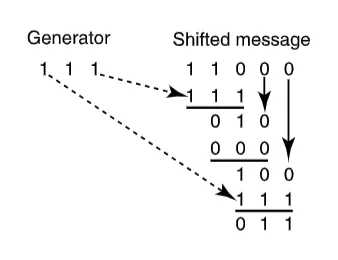
\includegraphics[width=0.75\textwidth]{../assets/ch02/ch02-2_7_1_差错检测和纠正-001.png}
    \caption{码距与检错纠错能力的几何直观。$d_{\min}=3$ 时可纠1位错误（两个纠错球不相交）；若只检错则可发现2位以内的错误。}
    \label{fig:hamming-distance}
\end{figure}

\subsection{奇偶校验：最简单的检错}

奇偶校验是在 $k$ 位数据后附加 1 位校验位，使整个 $k+1$ 位码字中"1"的个数为偶数（偶校验）或奇数（奇校验）。

以偶校验为例，发送数据 $1011001$（有4个1），校验位取0，发送 $10110010$；若发送 $1001001$（有3个1），校验位取1，发送 $10010011$。

接收方重新统计"1"的个数，若奇偶性不符，则检出错误。

\textbf{奇偶校验的局限}是显而易见的：它的最小码距为2，只能检测奇数个错误。两位同时翻转会让奇偶性恢复，错误就悄悄溜走了。因此，奇偶校验通常用于误码率很低、偶发单比特错误的场景，如内存校验（ECC 内存正是奇偶校验思想的扩展）和低速串口通信。

对于突发错误（burst error，即连续多个比特受同一个干扰影响而出错），奇偶校验几乎无能为力。需要更强大的机制。

\subsection{循环冗余校验（CRC）}

CRC 是现代数据通信中最广泛使用的差错检测方案。从以太网帧到 USB 数据包，从 ZIP 文件到卫星通信，CRC 无处不在。它强大的原因在于一个优雅的数学结构：\textbf{多项式除法}。

\subsubsection{CRC 的基本思想}

发送方和接收方事先约定一个\textbf{生成多项式} $G(x)$，其二进制表示称为生成串 $G$，长度为 $r+1$ 位（最高位和最低位均为1）。

设原始数据 $M$ 有 $k$ 位，CRC 的编码过程如下：

\begin{enumerate}
    \item 在 $M$ 后面附加 $r$ 个0，构成 $M' = M \cdot 2^r$（等价于将 $M$ 左移 $r$ 位）
    \item 用 $G$ 对 $M'$ 做\textbf{模2除法}，得余数 $R$（$r$ 位）
    \item 将 $R$ 替换掉 $M'$ 末尾的那 $r$ 个0，得到发送帧 $T = M' \oplus R = M' - R$（模2运算中加减等价）
\end{enumerate}

关键性质：$T$ 能被 $G$ 整除（模2意义下），即 $T \mod G = 0$。

接收方收到数据帧 $T'$（可能含错误）后，用同样的 $G$ 做模2除法。若余数为0，认为传输无误；若余数非零，确认发生了差错。

\subsubsection{为什么要用模2除法？}

模2运算（不进位的二进制加减法，等价于异或）是 CRC 的核心。它使得整个运算可以用线性反馈移位寄存器（LFSR）在硬件中极其高效地实现——每个时钟周期处理一位，成本几乎为零。

\subsubsection{CRC 的计算示例}

设 $M = 110$，生成串 $G = 111$（对应多项式 $x^2 + x + 1$，$r = 2$）。

\begin{enumerate}
    \item $M' = 11000$（$M$ 后追加2个0）
    \item 用模2除法计算 $11000 \div 111$：
\end{enumerate}

\[
\begin{array}{r}
    \phantom{0}110 \\
    111 \overline{)11000} \\
    \underline{111\phantom{00}} \\
    \phantom{1}100 \\
    \phantom{1}\underline{111} \\
    \phantom{11}11
\end{array}
\]

余数 $R = 11$，因此发送帧 $T = 11011$。

接收方收到 $11011$，做 $11011 \div 111$，余数为0，校验通过。若某位翻转，例如收到 $10011$，余数将不为0，立即检出差错。

\subsubsection{CRC 能检测哪些错误？}

选择合适的生成多项式 $G(x)$ 是 CRC 强大的关键。数学分析表明，一个精心设计的 $r$ 位 CRC 可以：

\begin{itemize}
    \item 检测所有单比特错误
    \item 检测所有两比特错误（只要 $G(x)$ 有至少3个因子）
    \item 检测所有奇数个错误（只要 $G(x)$ 含因子 $x+1$）
    \item 检测所有长度 $\leq r$ 的突发错误
    \item 以 $1 - 2^{-r}$ 的概率检测长度 $> r$ 的突发错误
\end{itemize}

这解释了为什么 CRC-32 在以太网中被采用：它对长度不超过32位的突发错误有100\%的检测率，对更长的突发错误仅有 $2^{-32} \approx 2.3 \times 10^{-10}$ 的漏检概率。

\subsubsection{常用 CRC 标准}

\begin{table}[htbp]
\centering
\caption{常用 CRC 标准及应用}
\begin{tabular}{llll}
\hline
\textbf{标准} & \textbf{多项式（Hex）} & \textbf{校验位} & \textbf{典型应用} \\
\hline
CRC-8       & \texttt{0x07}           & 8位  & I$^2$C 总线、传感器 \\
CRC-16-CCITT & \texttt{0x1021}        & 16位 & Modbus、USB、蓝牙 \\
CRC-32      & \texttt{0x04C11DB7}     & 32位 & 以太网、ZIP/PNG 文件 \\
CRC-64-ECMA & \texttt{0x42F0E1EBA9EA3693} & 64位 & 分布式存储、SCSI \\
\hline
\end{tabular}
\label{tab:crc-standards}
\end{table}

\subsubsection{CRC 与 TCP 校验和的分工}

实际网络中，一个 TCP 数据包同时携带两层差错保护：数据链路层的 CRC 和传输层的 TCP 校验和。这看似冗余，实则各司其职。

数据链路 CRC 在每一跳重新计算（因为链路帧头部每跳都变化），由网卡芯片硬件完成，擅长检测突发错误。但它无法捕捉路由器内部处理时引入的错误——一旦帧头重写，CRC 就被刷新了。

TCP 校验和覆盖端到端的完整路径，在软件中计算，用反码求和而非多项式除法（实现更简单），但检错能力弱于 CRC。两者互补，共同守护数据完整性——这是网络分层设计的一个典型案例：不同层次的机制解决不同范围的问题，不存在真正的"浪费"。

\subsubsection{CRC 的硬件实现}

CRC 运算的硬件实现极为优雅：用一个\textbf{线性反馈移位寄存器（LFSR）}，每个时钟周期移入一位数据，异或门放置的位置由生成多项式的系数决定。

\begin{figure}[htbp]
    \centering
    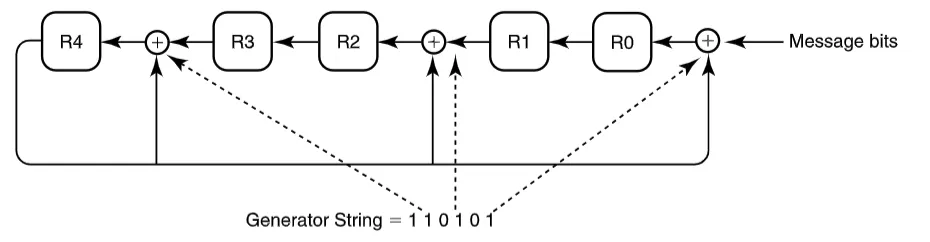
\includegraphics[width=0.85\textwidth]{../assets/ch02/ch02-2_7_1_差错检测和纠正-003.png}
    \caption{CRC 的 LFSR 硬件实现。寄存器 $R_4$ 的输出反馈到各个异或门，生成多项式系数为1的位置对应异或门。每个时钟周期移入一位，操作完成后寄存器中的内容即为 CRC 余数。}
    \label{fig:crc-lfsr}
\end{figure}

对于现代高速网络（100 Gbps 以上），逐位处理已不够快。实际实现会并行处理多位——利用查找表预计算中间结果，或用异或门矩阵一次完成 $W$ 位的 CRC 更新。

\subsection{汉明码：向纠错迈进}

检测到错误后，有两种选择：请求重传（ARQ），或在本地纠正（FEC，前向纠错）。重传简单但需要往返时延；纠错开销更大但可以零延迟恢复。卫星通信、存储系统、光纤传输等场景倾向于使用前向纠错，因为重传代价高昂甚至不可行。

\textbf{汉明码}是最经典的纠错码，由 Richard Hamming 在 1950 年发明，能纠正单比特错误、检测双比特错误。

\subsubsection{汉明码的构造}

汉明码的核心思想是：用若干\textbf{校验位}覆盖不同的数据位子集，使得每个数据位都被多个校验位"看护"。当某位出错时，出错的校验位组合能精确指出是哪一位，就像几道"探照灯"交叉定位一样。

设数据位数为 $k$，校验位数为 $r$，需满足：
\begin{equation}
    2^r \geq k + r + 1
    \label{eq:hamming-condition}
\end{equation}

校验位放在位置 $1, 2, 4, 8, \ldots$（2的幂次）处，数据位填充其余位置。校验位 $p_i$ 覆盖所有编号二进制表示中第 $i$ 位为1的位置。

以7位汉明码 (7,4)（4个数据位，3个校验位）为例。设数据位为 $d_3 d_2 d_1 d_0$：

\begin{itemize}
    \item $p_1$（位1）覆盖位 1, 3, 5, 7（二进制最低位为1）：$p_1 = d_2 \oplus d_0 \oplus d_1$
    \item $p_2$（位2）覆盖位 2, 3, 6, 7（二进制第二位为1）：$p_2 = d_3 \oplus d_0 \oplus d_2$
    \item $p_4$（位4）覆盖位 4, 5, 6, 7（二进制第三位为1）：$p_4 = d_3 \oplus d_1 \oplus d_2$
\end{itemize}

接收方重新计算这三个校验位，若某位出错，三个校验位的"符合/不符合"状态构成3位二进制数，其值恰好等于出错位的编号——0表示无错，1到7指向对应位置。将该位取反即可纠正。

这就是汉明码的精妙之处：$r$ 个校验位构成 $r$ 位二进制数，能直接"读出"错误在哪里。

\subsubsection{汉明码的局限与扩展}

基本汉明码只能纠正单比特错误。对于要求更高的场景，有以下扩展：

\textbf{扩展汉明码（SECDED）}：再添加一个整体奇偶校验位，使码距从3提升到4。可以\textbf{纠正1位错误，同时检测2位错误}（Single Error Correction, Double Error Detection）。这是 ECC 内存采用的方案——服务器内存每72位（64位数据 + 8位校验）构成一个 ECC 码字，在内存读取时实时纠正单比特翻转，是云数据中心和高可靠系统的标配。

\textbf{BCH 码（Bose-Chaudhuri-Hocquenghem）}和\textbf{Reed-Solomon 码}是更强大的纠错码族，能纠正多个错误，广泛用于 NAND 闪存、深空通信和数字广播。闪存随着使用老化会产生越来越多的比特错误，企业级 SSD 通常采用 BCH 或 LDPC 码，能纠正每1024字节中数十个错误。

\subsection{工业实践：从理论到芯片}

差错控制技术在工业界经历了从软件到硬件的彻底迁移。

\textbf{以太网}：CRC-32 由网卡硬件计算，100 Gbps 的线速下每秒处理约 150 万个帧，每帧计算耗时不足百纳秒。现代以太网芯片（如 Broadcom Tomahawk 系列）将 CRC 引擎深度流水线化，与数据接收并行完成，不引入任何额外延迟。

\textbf{数据中心互联（DCI）}：400G 及更高速率的光互联引入了\textbf{前向纠错（FEC）}作为物理层标准——KR4-FEC（基于 Reed-Solomon）在 400GBASE-R 中强制开启，以换取更大的链路功率预算，允许使用更长的光缆或更差的光模块。这是一个典型的用算力换链路裕量的工程权衡。

\textbf{AI 训练集群的 RDMA 网络}：阿里巴巴、腾讯等公司在大规模 RDMA 网络中发现，传统以太网的链路层差错控制机制（PFC 暂停帧）在遇到拥塞时会造成大范围的流量阻塞（Head-of-Line Blocking）。为此，他们开发了精细化的差错与拥塞协同控制方案——在硬件层实现 CRC 快速丢包检测，同时在 RDMA 层做选择性重传，避免整个网络因一条流的错误而停顿。这是 AI 基础设施迫使数据通信理论向工程实践演进的生动案例。

\begin{figure}[htbp]
    \centering
    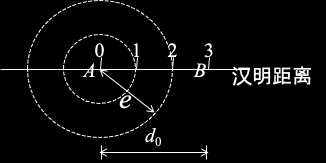
\includegraphics[width=0.85\textwidth]{../assets/ch02/ch02-2_7_1_差错检测和纠正-006.png}
    \caption{差错控制在协议栈各层的部署：物理层 FEC 对抗信道损伤，数据链路层 CRC 检测帧错误，传输层校验和提供端到端保护。各层机制互补，覆盖不同的错误场景。}
    \label{fig:error-control-layers}
\end{figure}
